
\chapter{Introduction and preliminaries} \label{chap:preliminaries}

Graph theory is the branch of computer science that focuses on the study of graphs. More broadly, it can be seen as the study of connections, since a graph represents the most general form of 'objects' and how they can be linked together.

The objects are referred to as nodes and are represented by points. These points are connected by edges, which are depicted as lines.   
\begin{center}
\begin{minipage}{0.5\textwidth} 
    \centering
    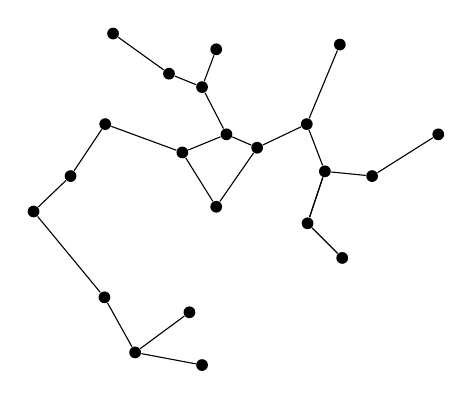
\begin{tikzpicture}[ every node/.style={circle, fill=black, inner sep=1.5pt}]

        
        \node (C) at (-1.03, -1.85) {};
        \node (D) at (-0.34, -1.34) {};
        \node (E) at (-0.18, -2.01) {};
        \node (F) at (0,0) {};
        \node (G) at (0.52,0.75) {};
        \node (H) at (1.15,1.05) {};
        \node (I) at (1.57,2.06) {};
        \node (J) at (1.38,0.45) {};
        \node (K) at (1.16,-0.21) {};
        \node (L) at (1.6, -0.65) {};
        \node (M) at (1.98,0.39) {};
        \node (N) at (2.82,0.92) {};
        \node (O) at (0.13,0.92) {};
        \node (P) at (-0.18,1.52) {};
        \node (Q) at (0,2) {};
        \node (R) at (-0.6,1.69) {};
        \node (S) at (-1.31,2.2) {};
        \node (T) at (-1.41,1.05) {};
        \node (U) at (-0.43,0.69) {};
        \node (V) at (-1.85,0.39) {};
        \node (W) at (-2.32,-0.06) {};
        \node (Z) at (-1.42,-1.15) {};

        \draw[-] (R) to (S);
        \draw[-] (R) to (P);
        \draw[-] (W) to (V);
        \draw[-] (T) to (V);
        \draw[-] (U) to (T);
        \draw[-] (W) to (Z);
        \draw[-] (Z) to (C);
        \draw[-] (D) to (C);
        \draw[-] (E) to (C);
        \draw[-] (K) to (J);
        \draw[-] (J) to (H);
        \draw[-] (I) to (H);
        \draw[-] (G) to (H);
        \draw[-] (O) to (G);
        \draw[-] (P) to (O);
        \draw[-] (Q) to (P);
        \draw[-] (U) to (F);
        \draw[-] (F) to (G);
        \draw[-] (J) to (K);
        \draw[-] (J) to (M);
        \draw[-] (M) to (N);
        \draw[-] (L) to (K);
        \draw[-] (O) to (U);
            
       
        
        % Collegamenti tra le stelle (archi non diretti)
      
        \end{tikzpicture}

\end{minipage}
\end{center}
\begin{definition}[Grafo]
    A graph $G = (N,E)$ is a structure composed of a set of nodes $N$
    and a set of edges $E$ that connect two nodes in  $N$
    \[(i,j) \in E \implies i,j\in N\]
    The set of nodes in a graph $G$ is denoted by $N(G)$, and similarly, the set of edges is denoted by $E(G)$. Often, the labels will be used to indicate the cardinality of these sets:
        \[\begin{array}{rcl}
            n &=& |N(G)|\\
            m &=& |E(G)| 
        \end{array}\]    
\end{definition}Various types of graphs exist in theory, just as various types of connections exist in the real world.
An edge can be:
\begin{itemize} 
    \item \textbf{directed}, to assign a direction to the connection
    \item \textbf{undirected}, indicating that the connection can be traversed in both directions.
\end{itemize} 

There are also \textbf{simple graphs}, where no more than one edge connects the same two nodes and no edges start and end at the same node, and \textbf{multigraphs}, where such edges are allowed.

Sometimes it is easy to see how something can be represented as a graph, other times the connection is more abstract.

Graph theory originated in 1736 with the Swiss mathematician Leonhard Euler. Euler wanted to know if it was possible to cross all the bridges of the city of Königsberg in a single walk, without crossing the same bridge twice.
\begin{center}
    \begin{minipage}{0.45\textwidth}  % larghezza per il grafo
        \centering
        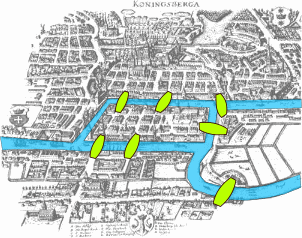
\includegraphics[width=\textwidth]{resources/images/Konigsberg_bridges.png}  % Percorso all'immagine
      \end{minipage}
      \!
      \begin{minipage}{0.45\textwidth}  % larghezza per l'immagine
        \centering
        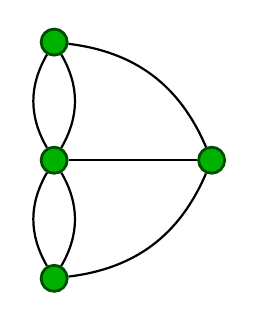
\begin{tikzpicture}[node distance={18mm}, thick, main/.style = {draw = green!30!black, circle, fill=green!70!black, line width=1pt}
            ] 
            \node[main] (0) at (-2, 0) {$ $}; 
            \node[main] (1) at (-2, 1.5) {$ $};
            \node[main] (2) at (-2, -1.5) {$ $};
    
            \node[main] (3) at (0,0) {$ $};
        
            \draw[-] (0) to [bend left] (1);
            \draw[-] (0) to [bend right] (1);
        
            \draw[-] (0) to [bend right] (2);
            \draw[-] (0) to [bend left] (2);
    
        
            \draw[-] (2) to [bend right] (3);
            \draw[-] (1) to [bend left] (3);
        
            
            \draw[-] (0) to  (3);
    
    
        
        \end{tikzpicture}   % Percorso all'immagine
      \end{minipage}
\end{center}

\begin{definition}
    A \textbf{walk} is an ordered sequence of edges where each edge starts from the node where the previous one ends (except for the first edge, of course).

    A \textbf{path} is a walk in which no node is visited more than once.
    \[P := \{(n_0, n_1),(n_1, n_2), ..., (n_{k-1}, n_k) \}\implies \nexists (a,b), (c,d)\in P | a = c \lor b = d\]
    
    A \textbf{circuit} is path that begins and ends at the same vertex.

\end{definition}

    In this case, the bridges can be represented as a multigraph where two distinct edges connect the same nodes.

\begin{definition}[Degree of a node]
    The degree of a node refers to the number of edges incident to that node.  
    
    In directed graphs, we can also distinguish between the out-degree and in-degree of a node, depending on the direction of the edges adjacent to it.
\end{definition}

In the end, Euler concluded that, for a graph to have an Eulerian path, it must have zero or two nodes with an odd degree, while for an Eulerian circuit, all nodes must have an even degree. With this, he demonstrated that the bridges of Königsberg do not have an Eulerian path, paving the way for the study of the potential of graphs.
\newpage
\section{Network and flow}
Nowadays, connections are expanding at an ever-increasing pace, forming networks that are becoming larger and more complex, whether physical or virtual. For this reason, from this point forward, we will focus on a specific type of graph: the network. We will analyze its properties and challenges in order to address various problems as efficiently as possible.
\begin{definition}[Network]
    In graph theory a network is a structure composed of a graph $G = (N,E)$ and a function $u: E \rightarrow \mathbb{N}^+\cup \{+\infty\}$ which denotes the capacity of each edge.
    \[u(i,j) = \text{capacity of the edge } (i,j)\]
    \begin{center}
        \textit{we will denote the capacity $u(i,j)$ below with the abbreviation $u_{ij}$}
    \end{center}
\end{definition}

When we refer to the capacity of an edge, we are talking about the maximum amount of flow that can pass through it.

In real-world applications, \textit{flow} can represent different things, such as the transfer of data in a network, the flow of water through a pipe, or even traffic flow on a road. The concept is versatile and applies to a wide range of scenarios depending on the context.

In each network exists two special nodes, s \textit{the source} and t \textit{the sink}. The network aims to send a certain \textbf{flow} from the source to the sink.
The edges in a network are directed, and except for $s$ and $t$, for all $(i,j)$ in a network $G$, $(j,i) \in E(G)$. We assume that the source $s$ has no incoming edges, just as the sink $t$ has no outgoing edges.
When representing two nodes in a network where the flow can only be routed in one direction, we can set the capacity of the flow in the opposite direction to zero.
Note that $u(i,j)$ refers specifically to the capacity of the edge from $i$ to $j$, and the capacity from $j$ to $i$ may be different.

\begin{figure}[h]
    \centering
    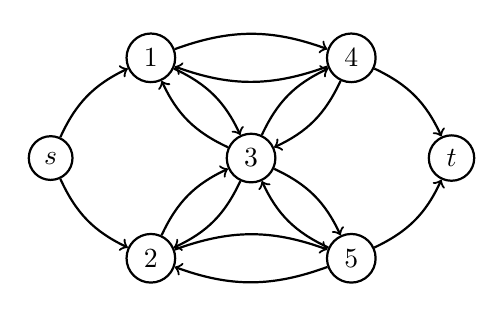
\begin{tikzpicture}[node distance={18mm}, thick, main/.style = {draw, circle}] 
        \node[main] (0) {$s$}; 
        \node[main] (1) [above right of=0] {$1$};
        \node[main] (2) [below right of= 0] {$2$};
        \node[main] (3) [above right of = 2] {$3$};
        \node[main] (4) [above right of=3] {$4$};
        \node[main] (5) [below right of=3] {$5$};
        \node[main] (6) [below right of=4] {$t$};
        
    
    
        \draw[->] (0) to [bend left = 20] (1);

    
        \draw[->] (0) to [bend right = 20] (2);

    
        \draw[->] (2) to [bend left= 20] (3);
        \draw[->] (3) to [bend left= 20] (2);
    
        \draw[->] (1) to [bend left= 20] (3);
        \draw[->] (3) to [bend left= 20] (1);

        \draw[->] (4) to [bend left= 20] (3);
        \draw[->] (3) to [bend left= 20] (4);

        \draw[->] (5) to [bend left= 20] (3);
        \draw[->] (3) to [bend left= 20] (5);

        \draw[->] (1) to [bend left= 20] (4);
        \draw[->] (4) to [bend left= 20] (1);


        \draw[->] (4) to [bend left= 20] (6);

        \draw[->] (5) to [bend left= 20] (2);
        \draw[->] (2) to [bend left= 20] (5);

        \draw[->] (5) to [bend right= 20] (6);

    
    \end{tikzpicture} 
    \caption{A classic example of a network}
\end{figure}



\begin{definition}[$U_{min},\ U_{max}$]
    In each Network we define:
    \begin{itemize}
        \item $U_{min}$: the smallest non zero capacity associated to an edge:
        \[U_{min} = u_{ij} | (i,j) \in E\ \land\ u_{ij} > 0\ \land\ \nexists (k,l) \in E : 0<u_{kl}<u_{ij}\]
        \item $U_{max}$: the largest finite capacity
        \[U_{max} = u_{ij}| (i,j) \in E\land u_{ij} \not = + \infty\ \land \]
        \[\nexists (k,l) \in E : u_{ij}< u_{jl} < +\infty \]
    \end{itemize}
\end{definition}
Moreover, we divide the edge into two categories:\\
\textbf{External Arcs} := $\{(x,y) | (x,y)\in E \land (x = s \lor y = t)\}$\\
\textbf{Internal Arcs} := $\{(x,y) | (x,y)\in E \land x \not = s \land y \not = t\}$ i.e. $E \setminus External\ edges$\\
\\
For our simplicity, we assume that for each internal edge $(i,j)\in E$ exists the edge $(j,i) \in E$.\\ The same thing is true for any internal node for which there always exists an edge that link it with $s$ and $t$, even if it has zero capacity.
\[\forall i \in N \implies \{(s,i),(i,t)\} \subseteq E\]

We can now give a formal definition of flow and the properties that it has to respect.
\begin{definition}[Flow]
    We define the flow as the function $f: E \rightarrow\mathbb{R}_+ \cup \{0\}$ which associates to each edge the amount of flow that is routed through.
    A flow function must satisfy the \textbf{flow conservation role}:
    \[\sum_{j:(i,j) \in E} f_{ij} - \sum_{j:(j,i) \in E}f_{ji} = 0 \quad \forall i \in N\setminus\{s,t\}\]
    that ensures us that there is no loss of flow as there are no unexpected entries.
\end{definition}

We call a flow \textit{feasible} if it respects the \textbf{capacity constraint}: \[\forall (i,j) \in E,\ f_{ij} \le u_{ij}\]

\begin{definition}[Flow value]

The \textbf{value of a flow} is given by the sum of all the outgoing edges of $s$ (or by the sum of all the incoming edges of $t$; it is the same)   
\end{definition}

\[val(f) = \sum_{\forall (s,x) \in E(G)} f_{sx} = \sum_{\forall (y,t) \in E(G)} f_{yt}\]
\begin{definition}[Residual capacity]
    The residual capacity of an edge $(i,j)$ means the amount of flow we can route in this edge before we saturate it.
    \[r_{ij} = u_{ij} + f_{ji} - f_{ij}\]    
    When we talk about residual capacity according to different flows we could also use the notation:    \[u_f(i,j)\]
    that means the residual capacity of the edge $(i,j)$ which has routed the flow $f$.

\end{definition}
We will often talk later about the residual function or the array of residual capacities, in fact we are referring to any function or structure that associates each arc with its residual capacity.

\begin{definition}[Residual Graph]
    Given a network $G$ and a flow $f$, we can define a residual graph as follows
    \[G[r] := (N(\mc{N}), \{(i,j) | (i,j)\in E(\mc{N}) \land r_{ij} > 0\})\]
    The notation $G[r]$ refers to a graph designed from the residual capacity function $r$. We will refer to the residual graph also using the notation $G_f$ that underlines the representation of the original network under the effect of the routed flow $f$
\end{definition}

\begin{definition}[s-t Cut]
    Given a network $G$ we define an $s$-$t$ cut on G as a partition into two subsets $(S, T)$ such that:
    \begin{enumerate}
        \item $s \in S$
        \item $t \in T$
        \item $S \cap T = \varnothing$
        \item $S \cup T = N$
    \end{enumerate}
    
    The \textit{cutting capacity} is defined as:
    \[u(S,T) = \sum_{i\in S\land j\in T} u_{ij}\]
    the \textit{residual of a cut} is defined as:
    \[r(S,T) = \sum_{i\in S\land j\in T} r_{ij}\]
\end{definition}

\begin{lemma}[Max residual flow min residual cut]
    \label{maxFlowMinCut}
    Given a residual graph $G[r]$ and a cut (S,T) then $r(S,T)$ represents the upper bound of the flow from $s \rightarrow t$.
In particular, the maximum increase in flow with respect to $r$ is the smallest residual capacity of an s-t cut.
\end{lemma}
\textit{Proof. }Omitted.\\

The lemma states that the problem of finding the maximum flow on a network is \textbf{dual} to that of finding a minimum capacity cut on the same network since this will represent the bottleneck that acts as an upper bound to the increase in flow.

\newpage
\begin{definition}(Anti-symmetric subset)
    Let $E(j)$ be de set of edges incident to a node $j$, we define the \textit{Anti-symmetric} subset of $j$ as:
    \[E'(j) :=\{(x,y)|(x,y)\in E(j) \land (x,y) \in E'(j) \iff (y,x) \not\in E'(j)\}\] 
\end{definition}

\textbf{Example:}\\
\begin{center}
    
\begin{tabular}{cc|cc}
    $E(j)  $&\qquad &\qquad& $E'(j)  $\\
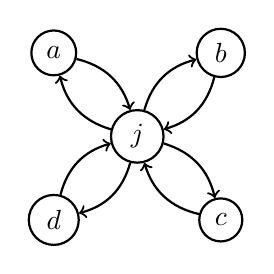
\begin{tikzpicture}[node distance={15mm}, thick, main/.style = {draw, circle}] 
    \node[main] (1) {$j$}; 
    \node[main] (2) [above right of=1] {$b$};
    \node[main] (3) [below right of=1] {$c$};
    \node[main] (4) [above left of=1] {$a$};
    \node[main] (5) [below left of=1] {$d$};


    \draw[->] (2) to [bend left] (1);
    \draw[->] (1) to [bend left] (2);

    \draw[->] (3) to [bend left] (1);
    \draw[->] (1) to [bend left] (3);

    \draw[->] (4) to [bend left] (1);
    \draw[->] (1) to [bend left] (4);

    \draw[->] (5) to [bend left] (1);
    \draw[->] (1) to [bend left] (5);

\end{tikzpicture} 
&&
&
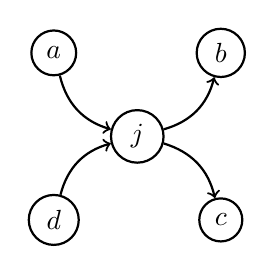
\begin{tikzpicture}[node distance={15mm}, thick, main/.style = {draw, circle}] 
    \node[main] (1) {$j$}; 
    \node[main] (2) [above right of=1] {$b$};
    \node[main] (3) [below right of=1] {$c$};
    \node[main] (4) [above left of=1] {$a$};
    \node[main] (5) [below left of=1] {$d$};



    \draw[->] (1) to [bend right] (2);


    \draw[->] (1) to [bend left] (3);

    \draw[->] (4) to [bend right] (1);


    \draw[->] (5) to [bend left] (1);


\end{tikzpicture} 
\end{tabular}
\end{center}
\begin{lemma}[Anti-symmetriy lemma]

    Given $E'(j)$ an anti-symmetric subset of $E(j)$ and a flow $f$ on $G$ with $r = r[f]$ then is true that:
    \[\sum_{(i,j)\in E'(j)}r_{ij} - \sum_{(j,i)\in E'(j)}r_{ji} = \sum_{(i,j)\in E'(j)}u_{ij} - \sum_{(j,i)\in E'(j)}u_{ji} \]
\end{lemma}
\begin{proof}
    \[\sum_{(i,j)\in E'(j)}r_{ij} - \sum_{(j,i)\in E'(j)}r_{ji} -\sum_{(i,j)\in E'(j)}u_{ij} + \sum_{(j,i)\in E'(j)}u_{ji}= 0 \implies\]
    \[\sum_{(i,j)\in E'(j)}(u_{ij}-r_{ij}) + \sum_{(j,i)\in E'(j)}(u_{ji}-r_{ji}) = 0 \]
    since $r_{ij} = u_{ij} - f_{ji} + f_{ij} \implies u_{ij} -r_{ij} = f_{ji}- f_{ij}$ 
    \[\sum_{(i,j)\in E'(j)}(f_{ji}-f_{ij}) + \sum_{(j,i)\in E'(j)}(f_{ij}-f_{ji}) = \sum_{(i,j)\in E(j)}(f_{ji}-f_{ij}) = 0\]
    so we deduce the conservation flow constraint. 
    \QED
\end{proof}
\section{Decomposition e transferring del flow}

\begin{definition}[Flow decompositon]
    Given $f$ an $s$-$t$ flow on a Network $\mc{N}$, we define a \textit{flow-decomposition}, as a collection of $s$-$t$ directed path 

    \[P_1, ..., P_k\quad where\ k < m\]
    To each path $P_i $ corresponds a value $\phi_i \in \mb{N^+} | \phi_i > 0$ that is the value of the path flow.

    In a flow decomposition the following rules must be respected: 
    \begin{enumerate}
        
        \item $\forall P_i, P_j,\  |P_i\cap P_j|\not = |P_i|\land |P_i\cap P_j|\not = |P_i|$ So each path in the decomposition must differ for at least one edge
        \item $ val(f) = \sum_{i = 1}^k \phi_i$
    \end{enumerate}


\end{definition}
An intuitive observation is that the maximum number of decompositions of any flow is $m$.\\
\begin{center}
    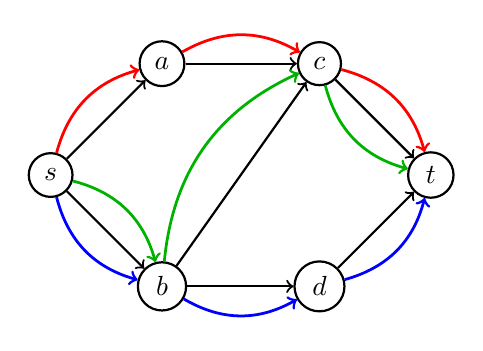
\begin{tikzpicture}[node distance={20mm}, thick , main/.style = {draw, circle}] 
    \node[main] (1) {$s$}; 
    \node[main] (2) [above right of=1] {$a$};
    \node[main] (3) [below right of=1] {$b$};
    \node[main] (4) [right of=2] {$c$};
    \node[main] (5) [right of=3] {$d$};
    \node[main] (6) [above right of=5] {$t$};
    %Admissible
    \draw[->] (1) to (2);
    \draw[->] (1) to (3);
    \draw[->] (3) to (5);
    \draw[->] (2) to (4);
    \draw[->] (5) to (6);
    \draw[->] (4) to (6);
    \draw[->] (3) to (4);
    
    %paths
    \draw[->,line width=1 pt] (1)[red, bend left] to (2);
    \draw[->,line width=1 pt] (2)[red, bend left] to (4);
    \draw[->,line width=1 pt] (4)[red, bend left] to (6);

    \draw[->,line width=1 pt] (1)[blue, bend right] to (3);
    \draw[->,line width=1 pt] (3)[blue, bend right] to (5);
    \draw[->,line width=1 pt] (5)[blue, bend right] to (6);

    \draw[->,line width=1 pt] (1)[green!70!black, bend left] to (3);
    \draw[->,line width=1 pt] (3)[green!70!black, bend left] to (4);
    \draw[->,line width=1 pt] (4)[green!70!black, bend right] to (6);

\end{tikzpicture} \\
Example of a decomposed flow 
\end{center}

Once we establish what decomposing a flow means, we can talk about capacity transfer
\begin{definition}[Tranfer]
    Given an edge $(i,j) \in E$ and a $path\ P\ i\rightarrow j$ with $|P|\ge 2$, \textbf{to transfer} $\delta$ unity of capacity from $P$ to $(i,j)$ means subtracting $\delta$ unity of residual capacity from each edge in $P$ and incrementing the $(i,j)$ residual capacity of the same $\delta$ unity
\end{definition}
\begin{lemma}[Capacity tranfer lemma]
    Let $P$ be $path$ in $G$ from node $i$ to node $j$ and let $(S,T)$ be an $s$-$t$ cut. 
    If we transfer delta capacity from the path $P$ to de edge $(i, j)$ and $r$ and $r'$ are respectively the residual capacity of the network before and after the transfer then is true that:
    \[r'(S,T) \le r(S,T)\] 
\end{lemma}
\begin{proof}
    The proof is trivial if $i,j \in S \lor i,j \in T$ since $u'(P) \le u(P) \implies u'(S,T)\le u(S,T)$.\\
    Otherwise if $i\in S \land j \in T$, if we consider $(l,k)\in P$ such that $l \in S\land k\in T$ we estimate
    \[u'(S,T)-u(S,T)\le (u'_{kl}+u'_{ij})- (u_{kl}+u_{ij}) = -\delta + \delta = 0\]
\end{proof}


\[\begin{tabular}{c|c}
    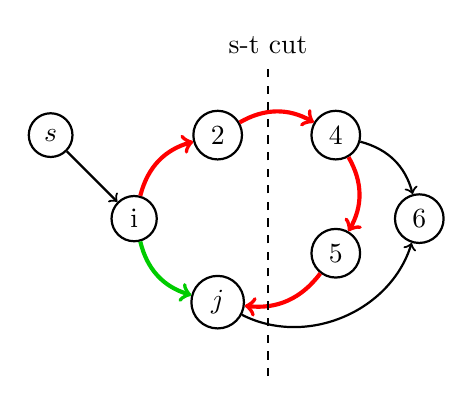
\begin{tikzpicture}[node distance={15mm}, thick , main/.style = {draw, circle}] 
    % Disegna i nodi del grafo
    
    \node[main] (1) {i};
    \node[main] (0) [above left of = 1] {$s$};
    \node[main] (2) [above right of=1] {$2$};
    \node[main] (3) [below right of=1] {$j$};
    \node[main] (4) [right of=2] {$4$};
    \node[main] (6) [below right of=4] {$6$};
    \node[main] (5) [below of=4] {$5$};
    % Disegna gli archi orientati
    \draw[->] (0) to (1);
    \draw[->,line width=1.5 pt] (1)[red, bend left] to (2);
    \draw[->,line width=1.5 pt] (1)[green!80!black, bend right] to (3);
    \draw[->,line width=1.5 pt] (2)[red, bend left] to (4);
    \draw[->,line width=1.5 pt] (4)[red,bend left] to (5);
    \draw[->] (4)[bend left] to (6);
    \draw[->] (3)[bend right = 50] to (6);
    \draw[->,line width=1.5 pt] (5)[red,bend left] to (3);

    % Aggiungi una linea tratteggiata per dividere il grafo in due
    \draw[dashed] (1.7,-2) -- (1.7,2);
    \node at (1.7,2.2) {s-t\ cut};

\end{tikzpicture}& 
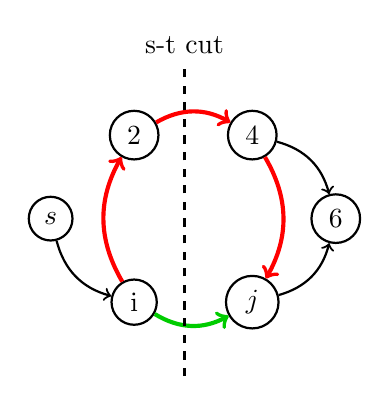
\begin{tikzpicture}[node distance={15mm}, thick , main/.style = {draw, circle}] 
    % Disegna i nodi del grafo
    
    
    \node[main] (0) {$s$};
    \node[main] (1) [below right of = 0] {i};
    \node[main] (2) [above right of=0] {$2$};
    \node[main] (4) [right of=2] {$4$};
    \node[main] (6) [below right of=4] {$6$};
    \node[main] (3) [below left of=6] {$j$};
    % Disegna gli archi orientati
    \draw[->] (0)[bend right] to (1);
    \draw[->,line width=1.5 pt] (1)[red, bend left] to (2);
    \draw[->,line width=1.5 pt] (1)[green!80!black, bend right] to (3);
    \draw[->,line width=1.5 pt] (2)[red, bend left] to (4);
    \draw[->,line width=1.5 pt] (4)[red, bend left] to (3);
    
    \draw[->] (4)[bend left] to (6);
    \draw[->] (3)[bend right] to (6);


    % Aggiungi una linea tratteggiata per dividere il grafo in due
    \draw[dashed] (1.7,-2) -- (1.7,2);
    \node at (1.7,2.2) {s-t\ cut};

\end{tikzpicture}\\
    \multicolumn{2}{c}{in {\color{red}{red}} the path P, in {\color{green!80!black}{green}} the edge (i,j)}

\end{tabular}\]

At the end of this consideration, we can deduce that transferring capacity from a path to an edge doesn't increase the maximum routable flow in a network
\newpage
\section{Distance based}
We usually think about graphs composed of nodes linked by edges and measure the distance between two nodes $i$ and $j$ as the sum of the edges on the shortest path that brings from $i$ to $j$. That is true just because we don't specify the length of an edge then we assume that it is one. Instead, we can specify the length of each edge and still divide the nodes by labels, i.e. by the distance from a specific node. But in doing this we have to pay attention to some rules that allow us to achieve our goal.
First of all we need to establish what a valid distance labeling is:
\begin{definition}[Valid distance labeling]
    \label{VDL}
    Let $N$ be a Network, $f$ a feasible flow on $N$ and $l$ a function that takes as input an edge in $G$ and returns its \textit{length}.\\
    The \textbf{distance function} $d: N(G) \rightarrow \mathbb{N}$ is said \textbf{valid} with respect to the residual graph $G[r]$ if it satisfies the following properties 
    \begin{enumerate}
        \item $d(t) = 0$
        \item $d(i) \le d(j) + l((i,j))$
    \end{enumerate}
\end{definition}

\begin{obs}[Valid distance label property]
    A valid distance label, $d$, preserves the following properties:
    \begin{enumerate}
        \item $d(i)$ represents the \textit{lower bound} of the length of the shortest path from $i \rightarrow t$
        in the residual graph
        \item $d(s) \ge n \implies \nexists\ p\ path \in G[r]\ |\ p = s \rightarrow t $ 
    \end{enumerate}
    
\end{obs}
Another point of view of the second property that a valid distance label has to respect ($d(i) \le d(j) + l((i,j))$) is that:
\[\neg (d(v) > d(w) + l(v,w))\]
This means that can not exist a node $i$ that is more distant from $t$ than any node $j$ adjacent to $i$, plus the length of the edge $(i,j)$.

\begin{definition}[Admissible graph]
    \label{AdmissibleGraph}
    Let $G$ be a Network with a feasible flow $f$, a valid distance label $d: N(G_f) \rightarrow \mathbb{N}$ 
    and a length function $l$.
    A \textit{residual arc} is called \textbf{Admissible arc} if it satisfies:
    \[d(v) = d(w) + l(v,w) \quad \forall (v,w) \in E(G(f))\]
    i.e.
    \[d(v) > d(w) \lor (d(v) = d(w) \land l(v,w) = 0)\]
    The \textbf{Admissible graph} is the graph formed by all admissible arcs.
    We will represent the admissible graph with the notation $A(f,l,d)$ or just $A(f,d)$ if the length function is trivial.
\end{definition}


\begin{obs}{}{}
    Let $G_f$ be a residual graph, let $B_s$ be an arborescence given by a BFS on the graph $G_f$ from node $s$ and let $A$ l'\textit{admissible graph} of $G_f$ then
    \[E(B_s)\subsetneq E(A)\]
\end{obs}

\[
    \begin{array}{c|c|c}
        
    
    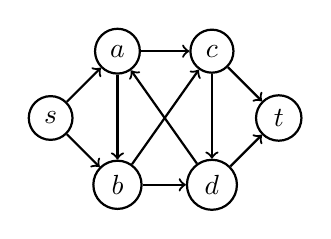
\begin{tikzpicture}[node distance={12mm}, thick , main/.style = {draw, circle}] 
    \node[main] (1) {$s$}; 
    \node[main] (2) [above right of=1] {$a$};
    \node[main] (3) [below right of=1] {$b$};
    \node[main] (4) [right of=2] {$c$};
    \node[main] (5) [right of=3] {$d$};
    \node[main] (6) [above right of=5] {$t$};
    %Admissible
    \draw[->] (1) to (2);
    \draw[->] (1) to (3);
    \draw[->] (3) to (5);
    \draw[->] (2) to (4);
    \draw[->] (5) to (6);
    \draw[->] (4) to (6);
    \draw[->] (3) to (4);
    \draw[->] (4) to (5);
    \draw[->] (5) to (2);
    \draw[->] (2) to (3);
\end{tikzpicture}  &
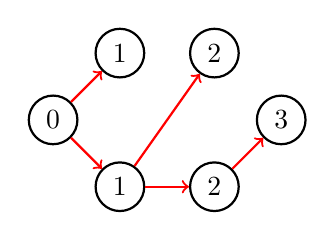
\begin{tikzpicture}[node distance={12mm}, thick , main/.style = {draw, circle}] 
    \node[main] (1) {$0$}; 
    \node[main] (2) [above right of=1] {$1$};
    \node[main] (3) [below right of=1] {$1$};
    \node[main] (4) [right of=2] {$2$};
    \node[main] (5) [right of=3] {$2$};
    \node[main] (6) [above right of=5] {$3$};
    %Admissible
    \draw[->, red] (1) to (2);
    \draw[->, red] (1) to (3);
    \draw[->, red] (3) to (5);
    \draw[->, red] (5) to (6);
    \draw[->, red] (3) to (4);
\end{tikzpicture} &
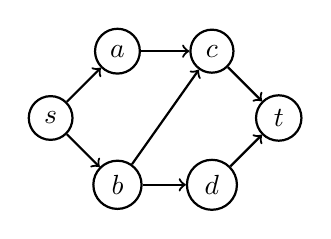
\begin{tikzpicture}[node distance={12mm}, thick , main/.style = {draw, circle}] 
    \node[main] (1) {$s$}; 
    \node[main] (2) [above right of=1] {$a$};
    \node[main] (3) [below right of=1] {$b$};
    \node[main] (4) [right of=2] {$c$};
    \node[main] (5) [right of=3] {$d$};
    \node[main] (6) [above right of=5] {$t$};
    %Admissible
    \draw[->] (1) to (2);
    \draw[->] (1) to (3);
    \draw[->] (3) to (5);
    \draw[->] (5) to (6);
    \draw[->] (3) to (4);
    \draw[->] (2) to (4);
    \draw[->] (4) to (6);
\end{tikzpicture} \\
\text{grafo originale}&\text{arborescenza} & \text{Admissible graph}
\end{array} 
\]
Given the distance label definition, we can recall the notions about s-t cut to define the \textbf{canonical cut}
\begin{definition}[Canonical cut]
    \label{cancut}
    Given a network $\mc{N}$ and a distance label $d$ on $\mc{N}$, a canonical cut is defined by a partition made as follows
    \[(S_k, T_k) =  (S_k:=\{v\in V(\mc{N}) | d(v) \ge k\},\ T_k := V(\mc{N})\setminus S_k)\]
\end{definition}

\section{Max flow}
To find the maximum flow in the network, we can use the \textbf{Edmonds-Karp algorithm}\cite{Edmonds_Karp}.

This algorithm finds the shortest path from the source to the sink $P$ and augments the flow on the edges of the path by the value $x$ s.t.
\[x = \min_{\forall (i,j)\in P} r_{ij}\]
In this way at each increment at least one edge is deleted from the residual graph and in at most $O(nm)$ increments the algorithm terminates.
Since we need $O(n+m)$ time to use the BFS to find the shortest s-t path and other $O(n)$ time tu augments flow in this path, Edmonds-Karp algorithm take $O(nm^2)$ time to find a maximum flow in any network.

Up to here, all notations that we need to recognize a network and its properties were given. The Edmonds-Karp algorithm represents the first step in a series of improvements that will lead us to find the max flow in $O(nm)$. From here on, each algorithm will bring a modification of the previous one while preserving the original intuition. The last algorithm shows how to reach the desired cost even for sparse graphs.

\cleardoublepage
